\chapter{Evaluation}
\label{chap:eval}
\section{Testing with Joystick}
\label{sec:evalJoystick}

In order to evaluate, at an early stage, how flyable and responsive to external commands the V-REP Quadcopter was, and how reliable the communication link between the V-REP and the Ivy-Bus system is, a Hardware-in-the-loop (HIL) set-up was build. 
\ref{fig:finkenHIL} shows the HIL set-up, consisting of a joystick, which is attached on the Ivy-Bus and controls the V-REP Quadcopter.


\begin{figure}[h!]
 \begin{center}
  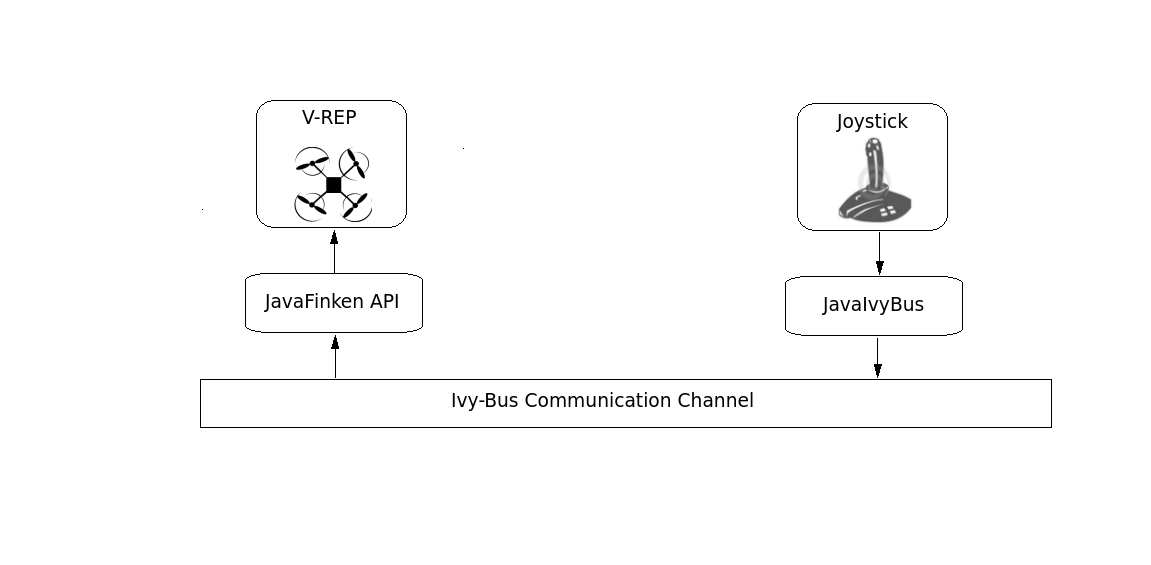
\includegraphics[scale=0.5]{FinkenHIL.png}
 \end{center}
  \caption{Finken Hardware-in-the-loop\label{fig:finkenHIL}}
\end{figure}

The HIL evaluation was implemented as a separate project - \textit{JavaFinkenSimHil}. 
It uses the Java external library \href{https://java.net/projects/jinput}{JInput} for reading the inputs from the joystick. 
The already created \textit{JavaIvyBus} module, which was discussed in \ref{sec:ivyBusImplementation}, is used to connect the Joystick to the Ivy-Bus. \\

The \textit{Joystick} class has as a local variable the class \textit{JoystickBusNode}, which extends the abstract \textit{AbsIvyBusNode}, thus being able to communicate on the common Ivy-Bus network. \\

The \textit{Joystick} class polls the data from the Joystick device at 50 MHz and sends them to the \textit{JoystickBusNode}, which on the other hand encapsulates the data in a FINKEN\_ROTORCRAFT\_FP message and publishes it on the bus. \\ 

The FINKEN\_ROTORCRAFT\_FP is the message that the real Quadcopter uses to publish its pitch, yaw and roll angles. 
Since the Joystick fakes the real Quadcopter, the JavaFinkenApp receives the message as if coming from the real one, thus not even a single line of code had to be changed in the JavaFinkenApp, in order to use the HIL evaluation. \\

As a result of the evaluation we came to the following conclusions:

\begin{itemize}
\item{The controlling of the Quadcopter was very precise and accurate. 
We ware able to make any maneuver and flight path as desired. \\ 

When flying with the Joystick, one can get a real feeling of the Quadcopter flight dynamics and behavior}.

\item{We experienced challenges with keeping the Quadcopter at a level height, using the throttle levers of the Joystick. 
It turned out, that keeping a level height was a matter of eye-hand coordination. \\

Even the slightest change to the thrust when hovering resulted in a strong acceleration in $z$-axis. 
Even if this behavior corresponds to the real quadcopter, we identified it as a problem, as the hover thrust of the real quadcopter changes during flight time with the battery voltage. 
As a result, we decided to tune the throttle response of the virtual Quadcopter with a logistic curve as described in \ref{equ:logistic}}.

\end{itemize}

\section{Simulation and Messaging  Performance}
\label{sec:performance}
\subsection{V-REP performance}
 The V-REP simulation is quite performant, running even on an old $2.4 GHz$ Core 2 Duo (T8300, 4GB RAM) close to real time.
 On this machine, running OS X, the execution of the Lua scripts takes the most time with typically $32ms - 42ms$.
 The distance sensor handling takes $14ms - 18ms$ and the Bullet physics engine accounts for $10ms — 12ms$.
 A modern computer even with a low-voltage i7 runs the simulation in real time without problems. A second computer, running Windows 10 with a i7-6650U CPU and 16GB RAM computes the Lua scripts in $26ms - 31ms$, the distance sensor handling in $6ms - 7ms$ and the Bullet physics in $6ms - 8ms$.
 These times are obtained by  the V-REP internal profiler.
 
 Profiling inside the Lua scripts showed, that the quadcopter main script, with the controllers and e.g. logging functions only takes 1-5 ms according to time measurements with  \emph{simGetSystemTimeInMs()}.
 The rotor scripts need $1ms - 5ms$ each, which might be optimizable.
 However, it seems that the biggest factor is the V-REP internal handling of Lua.
 Optimizing here might be possible, but requires detailed information about the internal structures.


 

\subsection{Timings in the Communication link}
\label{sec:commTiming}


The rate at which the V-REP simulated quadcopter receives the telemetry data from the flying quadcopter is crucial for the mixed reality simulation. 
The period at which a message is sent is configurable in the telemetry file, but there are several factors, that can influence the message frequency. 
The paparazzi ground station link module distributes the received telemetry on the Ivy-Bus and a slight delay could be expected there as a result of message buffering. 
The Ivy-Bus is a topic based publisher subscriber communication protocol and the processing of the regular expressions can be expensive. 
On the final link of chain is our Java communication bridge.\\

Considering the above factors, that can introduce a delay in the message transmission, we decided to measure how frequently the messages are sent to V-REP. 
Since V-REP does not provide any methods to measure the communication lag, we decided to measure how fast the Java communication bridge is sending the parameters to the V-REP. 
\ref{fig:messageLag} shows the results of the measurements with a single quadrocopter flying. 
The message is configured to be sent every 22 ms. 
What we see on the graph is that the average time at which the Java communication bridge sends the message to the V-REP quadcopter is around 27 ms. 
There are some messages that are sent even above 60 ms, but their number is relatively small and the delay scarcely exceeds the V-REP simulation step. 
A surprising fact is that some messages are sent even more frequently than the configured 22 ms. 
Since we could not find any explanation of this, we assumed that the paparazzi link uses some buffering strategy that leads to the observed fact. \\

In order to evaluate the performance of the Ivy-Bus when there are more agents, we did the same test with two flying quadrocopters. 
On \ref{fig:messageLag2} you can see that the graph shows the same pattern as in \ref{fig:messageLag}, but the average value is slightly increased.

\begin{figure}[h!]
 \begin{center}
  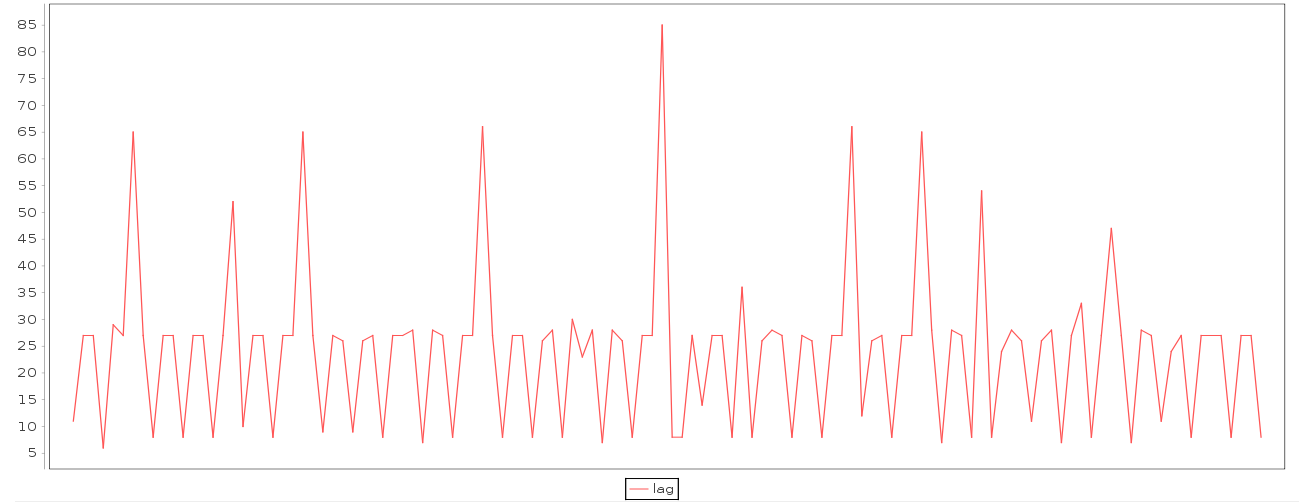
\includegraphics[scale=0.5]{messageLag.png}
 \end{center}
  \caption{message lag with one quadrocopter\label{fig:messageLag}}
\end{figure}

\begin{figure}[h!]
 \begin{center}
  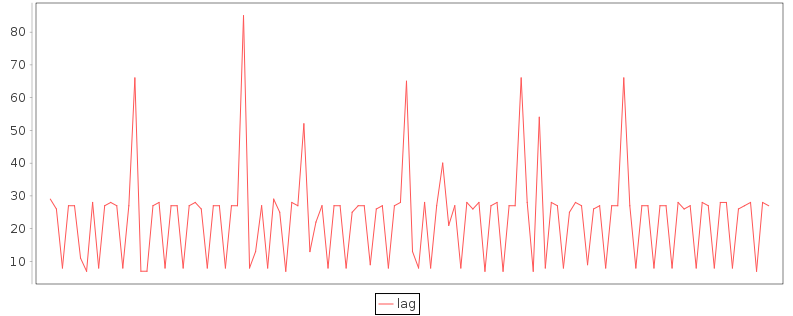
\includegraphics[scale=0.8]{messageLag2.png}
 \end{center}
  \caption{message lag with two quadrocopter\label{fig:messageLag2}}
\end{figure}



\section{Accuracy}
\label{sec:accuracy}
To evaluate the accuracy of the simulation, we compared the orientation of the real FINken and the simulated model.  
We let the real FINken fly freely in the arena using the wall avoid control and linked the simulated FINken.
V-REP, paparazzi and the Java bridge were all run on the same machine.
The test flight which is referred to in the following was filmed.
The video, a screen recording of the simulation and the corresponding log files can be found in the git repository of the project in \emph{./documentation/rawdata}, which is available in the working groups github environment.

The real quadcopter has some issues with the yaw angle. 
A cause for this is that the magnetometer does not provide reliable values indoors, due to interferences of electro-magnetic fields.
The sensors of the FINken are symmetrical, so yaw is not needed for regular movements.
Thus, it is tried to keep the copters orientation around the $z$ axis more or less stable.
The evaluation is described exemplary for one flight. 
Of course, this was not the only test that was run, but other experiments fortified the following results.

The pitch and roll angles of the simulated FINken are more interesting.
When we logged the values via the telemetry link of paparazzi, and compared them to the values exported from the simulation, we noticed a time offset. 
This is not surprising, as we don't use an absolute reference time, but it made it impossible to directly compare the orientation logs.
To get a meaningful graphic, we manually resampled the logs and put them on a common time base.
Characteristic patterns were used to achieve a common time base.
In \ref{pic:pitchResponse} can be seen that the simulated FINken nicely adopts the real FINken's movements. 
The first spike at about $7s$ shows the takeoff. 
From $12s$ to $22s$ it can be seen how the real FINken got close to a wall and started to avoid it. 
The flight was stopped after about $43s$, the huge spikes at the end of the graph show how the response when the copter fell to the ground.
\begin{figure}
	\begin{center}
	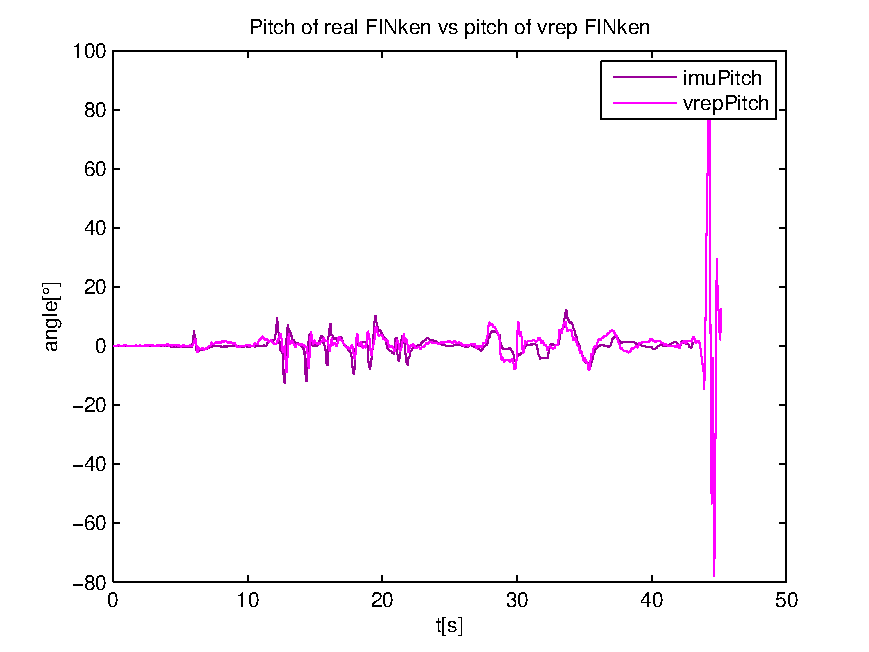
\includegraphics[width=\textwidth]{pitch}
	\caption{Pitch angles of simulated FINken and real FINken}
	\label{pic:pitchResponse}
	\end{center}
\end{figure}

The virtual copter started to drift away approximately at $30s$ as can be observed in the video.
In \ref{pic:pitchResponse} can be seen, that the virtual and real pitch deviate around $30s$ for a short time, which could be the cause for the drift.

A more detailed plot of the pitch comparison is shown in \ref{pic:pitchDetail}.
Every spike of the real FINken's movement is directly followed by a spike in the same direction of the simulated FINken.
The smaller movements do not correspond exactly, as the simulated copter contains its own attitude controller.
Thus, keeping the simulated FINken stable in air has a higher priority than following the real copter's movements.
The graph shows some points, e.g. before $17s$ where movement of the simulated FINken appears to precede the real FINken's movement.
This can have two possible explanations.
Firstly, as mentioned before, the time base was readjusted manually.
Thus, it might be possible, that as explained in \ref{sec:commTiming}, the values were sent with a wrong timestamp because of paparazzi's internal buffering.
If the wrong timestamps weren't corrected during the adjustment, or even made worse by the resampling ,they could shift the logged values.
Secondly,  the controller of the simulated FINken's controller has the same goal as the real FINken, namely to keep the copter stable. 
In the following, it could be possible, that both controllers are going to apply the same changes and that the virtual one is slightly faster.
 

\begin{figure}
	\begin{center}
	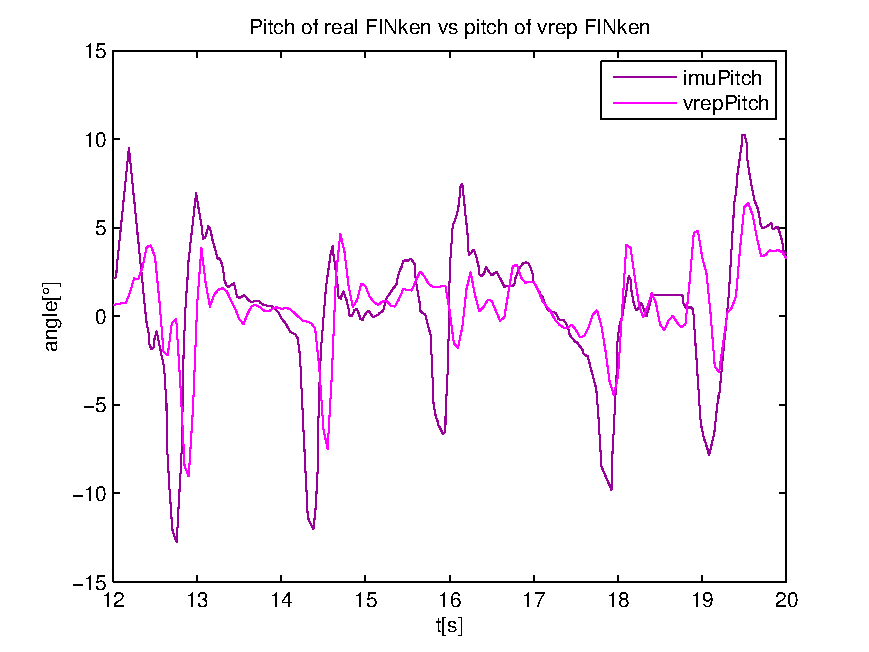
\includegraphics[width=\textwidth]{pitch_detail}
	\caption{Detailed pitch angles of simulated FINken and real FINken}
	\label{pic:pitchDetail}
	\end{center}
\end{figure}

Interestingly, the roll of the FINkens as shown in \ref{pic:rollResponse} doesn't fit as well as the pitch, despite having identical controllers.
In this flight, we observed some logging error in V-REP. 
The huge spikes in the virtual FINken's roll angle could not be observed in the screen capture of the simulation.
When comparing the spikes in \ref{pic:rollResponse} with the plot of the pitch in \ref{pic:pitchResponse}, one can notice that the erroneous spikes in the roll correspond to the valid spikes in the pitch.
An explanation could be, that the rotation matrix for the dummy object, which is linked to the simulated FINken's body, was not computed correctly.
Unfortunately, we could not reproduce this error, but it shows that one should be careful when using sensor data, be it from hardware sensors or from software.

\begin{figure}
	\begin{center}
	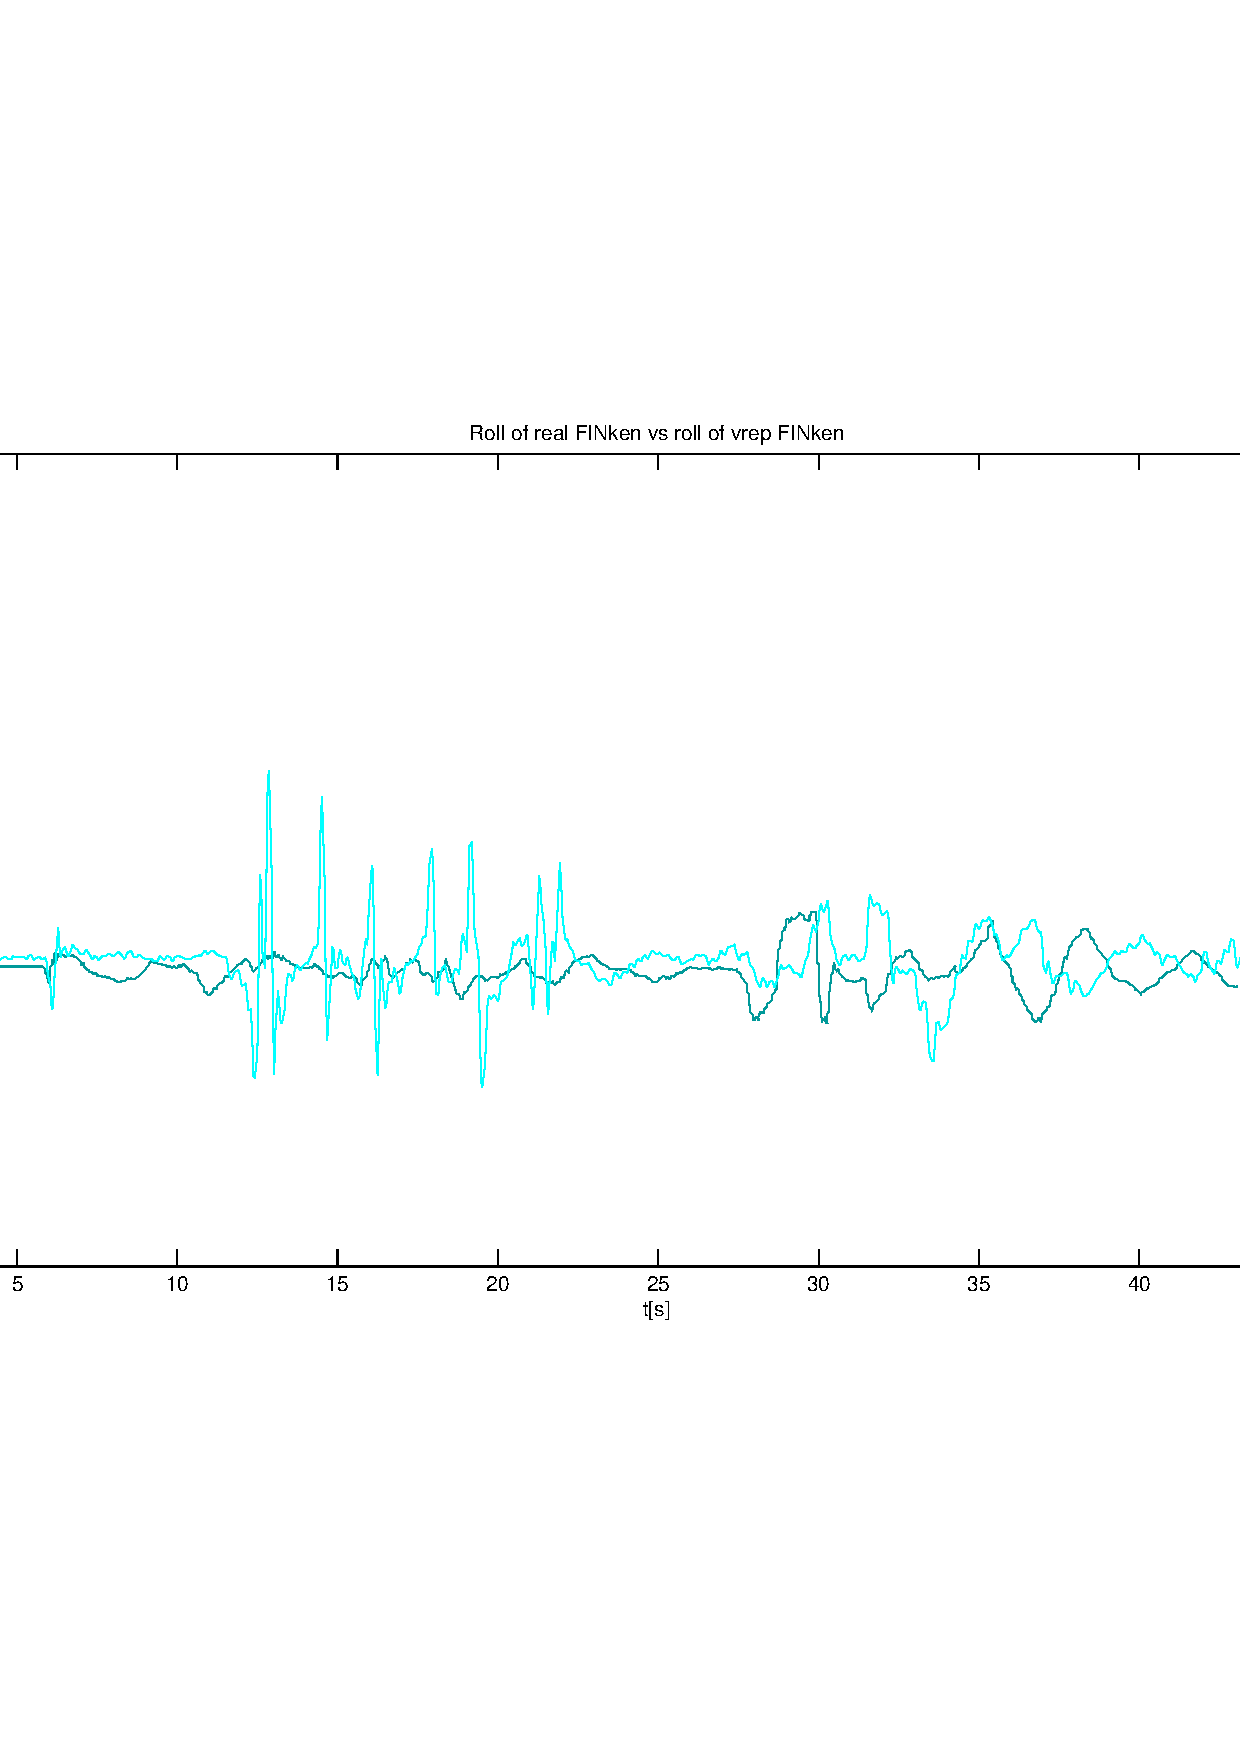
\includegraphics[width=\textwidth]{roll}
	\caption{Roll angles of simulated FINken and real FINken}
	\label{pic:rollResponse}
	\end{center}
\end{figure}

The plots for the angular responses of the simulation show, that it is possible to let a virtual FINken mimic a real flying one by transmitting the \gls{AHRS} values. 
The response of the model does not exactly match, but to achieve this, the simulation model needs to be excessively tuned, which is out of scope of this work.
\todo{plot difference between graphs}



Eventually we wanted to evaluate to what extend the path of the flying quadrocopter matches the path of the simulated quadcopter. V-REP provides an easy way to plot the two dimensional position of the quadrocopter and draw the flying path, but our real quadrocopter does not have a positioning system and its position estimation is not possible.\\ 

In order to estimate the position we have used the MEDUSA localization system developed in our faculty by Zug, Steup, Dietrich and Brezhnyev\cite{Zug2011RobLoc}. 
The system calculates the two dimensional position of a mobile robot moving in a rectangular arena, using eight proximity sensors and a gyroscope. 
It uses the yaw angle of the robot and the distances to the walls from the proximity sensors to calculate a set of possible positions, where the quadrocopter could be. 
Then it moves through all possible points and calculates the distances, that the proximity sensors should read at that particular point and angle of rotation. 
Comparing the real readings from the quadrocopter proximity sensors and the calculated distances, a probability function is calculated, that indicates the probability that the real quadrocopter is situated at the particular point. 
The point with the highest probability is chosen for the quadcopter position.\\

The MEDUSA positioning system turned out to be an easy and fast way to get an estimation of the position, since our quadcopter has four ultrasound sensors, positioned at 90 degrees from each other, and a gyroscope, which provides the angle of rotation. 
The fact, that the original positioning system uses eight distance sensors was not disturbing, since it is possible to estimate the position even with two sensors. 
But a higher number of sensors provides more fault-tolerance to the system and more accuracy. 
It was also not necessary to implement the algorithm in the firmware of the quadcopter. 
We used the log file, that the Paparazzi software uses to write the sensor data and fetch the sensor readings from there using a Matlab script. 
Only a minor changes ware required in the configuration of the sensor numbers, the sensors maximum range and the size of the arena.\\

On \ref{fig:matlabPosEstimation} you can see the calculated possible positions and the quadcopter positioned at the point with the highest possibility value. 
The lines represent the ultrasound sensors and the length of the lines depict the maximum sensor range. 
The red fractions of the lines show the actual distance measured by the sensor. 

\begin{figure}[h!]
 \begin{center}
  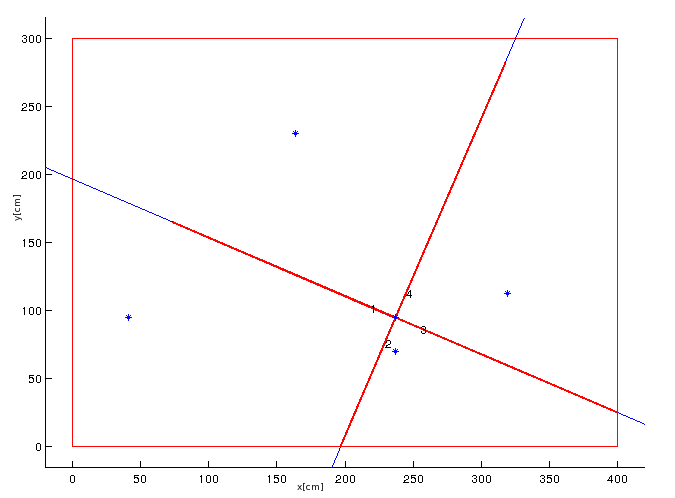
\includegraphics[scale=0.7]{MatlabPositionEstimation.png}
 \end{center}
  \caption{position estimation\label{fig:matlabPosEstimation}}
\end{figure}

The positioning system relies on accurate sensor readings to provide a precise position estimation. 
Our gyroscope provides noisy estimation of the yaw angle and the distance sensors are also quite noisy. 
Since our quadcopter is equipped with just four distance sensors, the localization system cannot tolerate the noise as good as with eight sensors. 
For this reasons an accurate position estimation could not be expected, but it should provide some reference estimation of the flying path. 
On \ref{fig:matlabPosPath} you can see the results of the position estimation. 
Each position has been marked with a blue star, so that we can see where the quadcopter has been. 
It is not possible to show the actual flying path as a function of time, but it shows which parts of the arena had been occupied by the quadcopter during the flight. 
\ref{fig:vrepPosPath} shows the flight path of the simulated quadcopter in the V-REP. 
As in \ref{fig:matlabPosPath} it does not shows the trajectory as a function of time, but just the occupied positions during the flight. 
The x and y axes of the plot show the V-REP scene arena and the small rectangle represents the flight arena.

\begin{figure}[h!]
 \begin{center}
  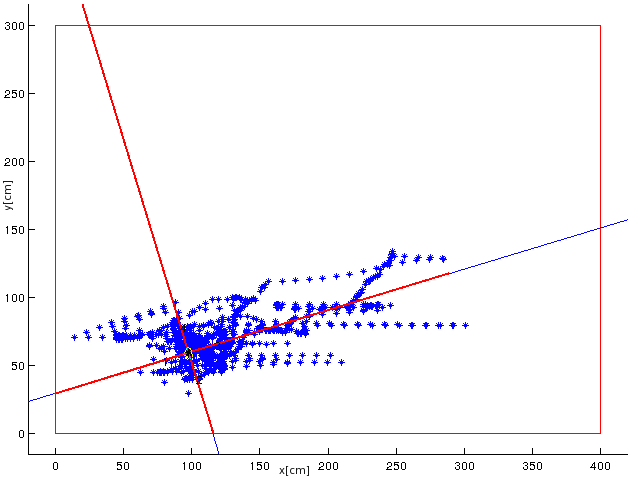
\includegraphics[scale=0.7]{MatlabPositionPath.png}
 \end{center}
  \caption{Estimated flight path\label{fig:matlabPosPath}}
\end{figure}

\begin{figure}[h!]
 \begin{center}
  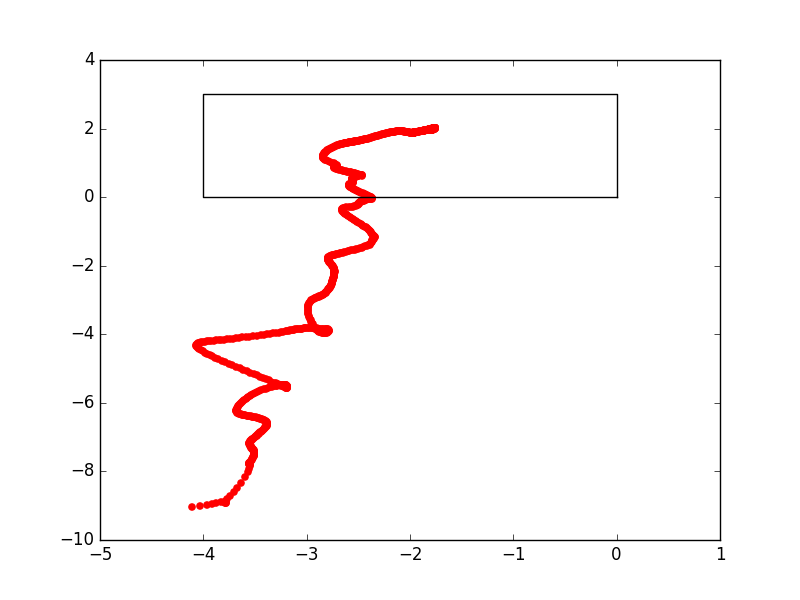
\includegraphics[scale=0.7]{vrepPath.png}
 \end{center}
  \caption{V-REP flight path\label{fig:vrepPosPath}}
\end{figure}

The estimated positions on \ref{fig:matlabPosPath} are very scattered, due to the fact that the localization system cannot estimate the position with a big accuracy. 
In the worst case, as a correct position was assumed one of the calculated possible points, which was far away from the previous estimated position. 
This creates a big jumps in the path, which does not coincide with the real flight path. 
The scattered plot and the jumps are caused by the noisy sensor measurements. 
A couple of attempts to filter the sensor readings ware made, but the plot still looked scattered to a significant extend. 
Thereupon, to eliminate the jumps, we limited the distance the copter could move in a single time step.
This resembles that the real FINken can only move with a limited velocity.
However, this improved the results slightly but still isn't satisfying for a perfectly accurate positioning system.


On the other hand \ref{fig:vrepPosPath} shows a clear flying path, due to the fact that the position is not estimated, but taken directly from the V-REP environment. 
The graph shows how the quadcopter drifts and to what extend it flies away from the arena.\\

Eventually we came to the conclusion, that the used approach for position estimation was not good enough for our needs and a detailed comparison between the flying paths of the real and simulated quadcopter could not be done at this stage. 
However the working group has the intention to build a camera positioning system and track the quadcopter position with a camera mounted on the top of the arena.


